\section{Methodology}
~\label{sec:methodology}
\hspace{12pt}
In this section, the project requirements and the following methodology are described.

\subsection{Project Requirements}
~\label{sec:methodology:project_reqs}
\hspace{8pt}

The design must include the following features:

\begin{enumerate}
    \item The system requires an analog sensor with a voltage, current, resistance, capacitance or inductance output, and a sensor that connects to a data bus (\acrfull{spi} or \acrfull{i2c}). The aim is for the application to be relevant, that is, to have a practical use. There are no restrictions regarding the different sensors being complementary (for example, measuring temperature). The sensors to be used, even if done theoretically, will be real sensors, and, therefore, must be based on the data sheets of each sensor chosen for the work and simulations. Selection of each of the sensors and justification must be given.

    \item Selection of data sample device. The system is intended to sample sensor values on some type of data sample device.

    \item Design of signal connectors, including their conditioning when necessary.

    \item Demonstrate, in the case of the analog sensor, that the conditioning is working properly (for example, the output voltage is correct). Choose a filter type, investigate its implementation, and justify the choice according to the application to be made. Take into consideration that amplifiers should not be considered ideal, and parameters must be configured. A virtual amplifier can be used, but its values must be configured concerning a real amplifier.

    \item Design of an algorithm for data collection. Take into consideration energy management modes when using the system.

    \item Design of the complete system at the connection level (that is, to understand it better, the design at a level that would allow proceeding to the design of a \acrfull{pcb}).
\end{enumerate}


\subsection{Developed Methodology}
~\label{sec:methodology:dev_methodology}
\hspace{8pt}
In this section, the selection of the sensors, the data sample device, and the design decisions are described. Also, the developed algorithm for data collection is shown.


\subsubsection{Sensors}
~\label{sec:methodology:dev_methodology:sensors}
\hspace{8pt}
First of all, the selected variables to measure the \acrshort{iaq} were the temperature, humidity, and gas concentrations. High temperatures can affect the exhaled CO$_{2}$ concentration, a harmful air pollutant, as well as an increase in the pulse rate~\cite{en14238127}. Some studies have shown a correlation between coarse particulate matter and relative humidity~\cite{yang_2020, tanatachalert_2023, xing_2016}. Humidity can affect particle concentration by influencing the formation, growth, and behavior of particles in the atmosphere, as well as the dispersion and transportation of such particles~\cite{tanatachalert_2023}. This particle concentration can cause respiratory symptoms--like coughing, wheezing, and shortness of breath--and cardiovascular problems--like atherosclerosis and heart attacks--with long-term effects~\cite{ahamed_2022, ding_2021, tang_2021}. \\

To measure those variables, the following sensors were selected:

\begin{itemize}
    \item \textbf{MQ-2 Gas Sensor:} It is an analog sensor designed to detect smoke and flammable gases. It is primarily utilized in home gas leak alarms and detectors due to its heightened responsiveness to propane and smoke. Some good characteristics of the MQ-2 sensor are~\cite{mq2_datasheet, components101_mq2}:

        \begin{enumerate}
            \item \textbf{\textit{Versatility:}} It is capable of detecting a variety of flammable gases and smoke making it useful for a range of applications in family and industry.

            \item \textbf{\textit{Sensitivity:}} It has high sensitivity to gases such \acrfull{lpg}, i-butane, propane, methane, alcohol, Hydrogen, making it ideal for air quality monitoring. As shown in the datasheet~\cite{mq2_datasheet}:

            \begin{itemize}
                \item 200ppm-5000ppm \acrshort{lpg} and propane.

                \item 300ppm-5000ppm butane.

                \item 5000ppm-20000ppm methane.

                \item 300ppm-5000ppm $H_{2}$

                \item 100ppm-2000ppm Alcohol
            \end{itemize}

            \item \textbf{\textit{Ease of use:}} It is easy to use and interface with microcontrollers like Arduino. It provides an analog output that can be read directly by an analog pin on the Arduino.

            \item \textbf{\textit{Availability:}} It is widely available and relatively inexpensive, making it an attractive option for many \acrfull{diy} projects and commercial applications.
        \end{enumerate}

    \item \textbf{BMP180 Barometric Pressure Sensor:} It is a high-precision sensor designed for consumer applications used to measure barometric or atmospheric pressure~\cite{components101_bmp180}. The BMP180 sensor senses that pressure and provides that information in digital output~\cite{bmp180_datasheet}. Since the temperature also affects the pressure, the BMP180 sensor has a good temperature sensor to compensate for pressure readings~\cite{components101_bmp180}. Some advantages of the BMP180 sensor are~\cite{components101_bmp180, bmp180_datasheet}:

        \begin{enumerate}
            \item \textbf{\textit{Versatility:}} It can measure both temperature and altitude, making it useful for various applications.

            \item \textbf{\textit{High Relative Accuracy:}} It has a high relative accuracy of $\pm0.12$hPa, making it reliable for precise measurements.

            \item \textbf{\textit{Low Power Consumption:}} It consumes very little power ($3\mu$A), making it ideal for battery-operated systems like smartwatches and mobile phones.

            \item \textbf{\textit{Fast Communication:}} It is capable of communicating with a high-speed \acrfull{twi} with a 3.4Mhz interface, making it suitable for applications where high-speed communication is needed.

            \item \textbf{\textit{Wide Operating Temperature Range:}} It can operate in a wide temperature range from $-40^{\circ}$C to $+80^{\circ}$C.
        \end{enumerate}
\end{itemize}


\subsubsection{Data Sample Device}
~\label{sec:methodology:dev_methodology:sensors:dsd}
\hspace{8pt}
Gas sensors can be affected by \acrfull{lfn} coming from different sources, including flicker noise (pink noise or 1/f noise) and thermal noise (Johnson-Nyquist noise)~\cite{Kwon_2014, wonjun_2023,smulko_2024}. \\

Flicker noise can be observed in various electronic devices and systems--including chemoresistive-based sensors--and it decreases as the frequency increases. In the context of gas sensing, resistance fluctuations in the sensing materials can be measured as low-frequency noise, typically up to a few kHz. The intensity and slope of the power spectral density of the flicker noise can enhance gas sensing capabilities. Different measurement setups and noise-processing methods are used for gas detection in resistive gas sensors, depending on the \acrfull{dc} resistance of the sensing materials~\cite{Kwon_2014, kiely_2017}. In well-designed systems, Flicker noise is generally the primary source at lower frequencies, whereas white noise tends to prevail at higher frequencies~\cite{bahreyni_2009}. In Fig~\ref{fig:flicker_noise_vs_frequency}, how a \acrfull{psd} of a system output looks like is shown~\cite{bahreyni_2009}.

\begin{figure}[ht]
    \centering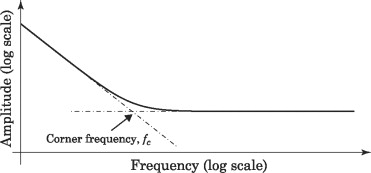
\includegraphics[width=0.6\linewidth]{flicker_noise_vs_frequency}
    \caption{A typical \acrshort{psd} for the noise at the output of a system in the presence of both Flicker and white noise sources.}
~\label{fig:flicker_noise_vs_frequency}
\end{figure}

The corner frequency (f$_{c}$) is the frequency at which the Flicker noise and the white noise of a system are equal in magnitude and is a key parameter in characterizing the noise performance of electronic devices~\cite{smulko_2024}. For the MQ-2 gas sensor specifically, it would need to conduct noise measurements and spectral analysis. This involves measuring the output voltage of the sensor over a range of frequencies and plotting the noise spectral density. Since this is out of the project scope, based on~\cite{smulko_2024} findings, a value of 50kHz is assumed for this project. Having said that a high-pass filter will be used to filter the noise of the signal. \\

Butterworth filter is characterized by a smooth roll-off and a flat response in the passband, which means that it attenuates frequencies outside the passband without introducing ripples or distortions~\cite{ruofei_2021}. This filter might not be the best choice for Flicker noise because of its maximally flat frequency response and Flicker noise is more prominent at lower frequencies, and a filter with a sharper cutoff might be more beneficial. Chebyshev filter is a type of \acrfull{iir} filter that provides a steeper roll-off in the stopband compared to Butterworth filter~\cite{podder_2014}. However, the passband ripples can cause additional noise. Bessel filter is a type of low-pass filter that exhibits a maximally flat frequency response in the passband, meaning that the magnitude response is nearly constant up to the cutoff frequency. They also have a linear phase response, meaning that all frequency components of the input signal are delayed by the same amount, preserving the waveform shape~\cite{ashu_2021}. In Fig~\ref{fig:butterworth_vs_chebyshev_vs_bessel_filters}, the comparison for the 3 filters is shown~\cite{kikkert_2008}. \\

\begin{figure}[ht]
    \centering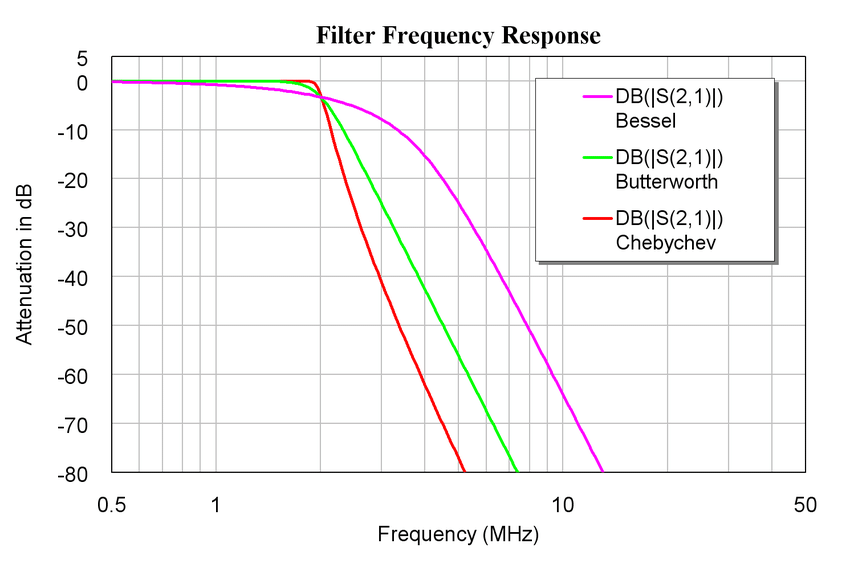
\includegraphics[width=0.8\linewidth]{butterworth_vs_chebyshev_vs_bessel_filters}
    \caption{Comparison of Butterworth, Chebyshev, and Bessel filters.}
~\label{fig:butterworth_vs_chebyshev_vs_bessel_filters}
\end{figure}

The filter to implement will be a second-order Bessel high-pass filter with a cut-off frequency of 50kHz. The Second-order filter was chosen to reduce the complexity of the designed system.

\newpage

\subsubsection{Signal Conditioning}
~\label{sec:methodology:dev_methodology:sc}
\hspace{8pt}
The diagram of the MQ-2 sensor can be obtained from its datasheet (Fig~\ref{fig:mq2_diagram})~\cite{mq2_datasheet}.

\begin{figure}[ht]
    \centering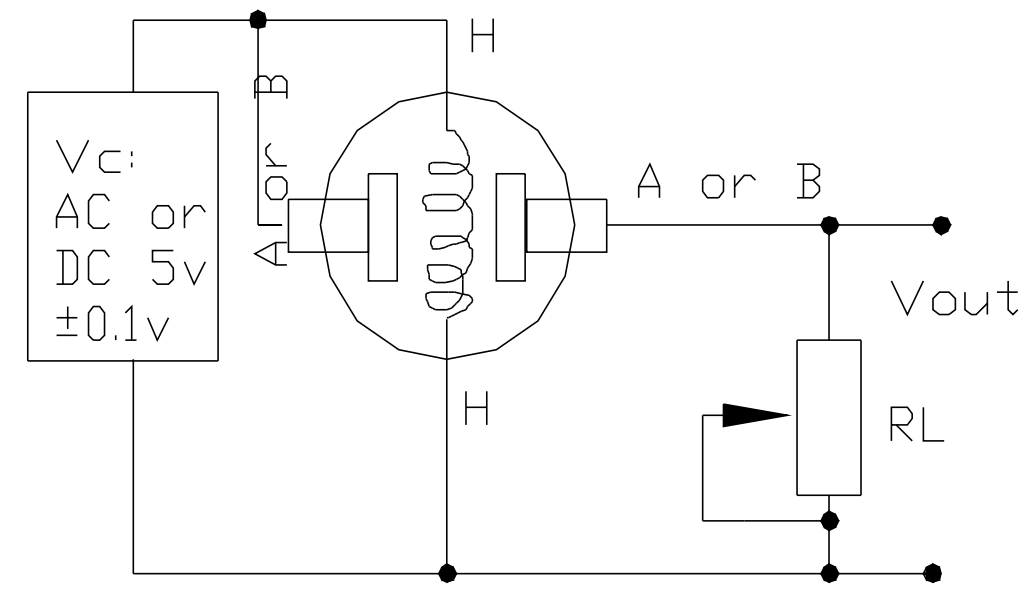
\includegraphics[width=0.5\linewidth]{mq2_diagram}
    \caption{MQ-2 sensor diagram.}
~\label{fig:mq2_diagram}
\end{figure}

The MQ-2 datasheet also mentions that the sensor requires calibration. For such a task, the manufactured provided the typical sensitivity characteristics of the MQ-2 for several gases--shown in Fig~\ref{fig:mq2_sensitivity_characteristics}. The values are set to:

\begin{itemize}
    \item Temp: 20$^{\circ}$C.

    \item Humidity: 65\%.

    \item O$_{2}$ concentration: 21\%

    \item R$_{L}$: 5k$\Omega$

    \item R$_{O}$: sensor resistance at 1000ppm of H$_{2}$ in the clean air.

    \item R$_{S}$: sensor resistance at various concentrations gases.

    \item V$_{C}$: circuit voltage (5V). \\
\end{itemize}

The output voltage V$_{out}$ is obtained from the voltage division of the load resistor R$_{L}$ (can adjust) and the sensor resistance R$_{S}$. Based on that:

\begin{equation}
    V_{out} = \frac{R_{L}}{R_{L} + R_{S}} V_{C}
    \label{eq:voltage_division}
\end{equation}

\begin{figure}[ht]
    \centering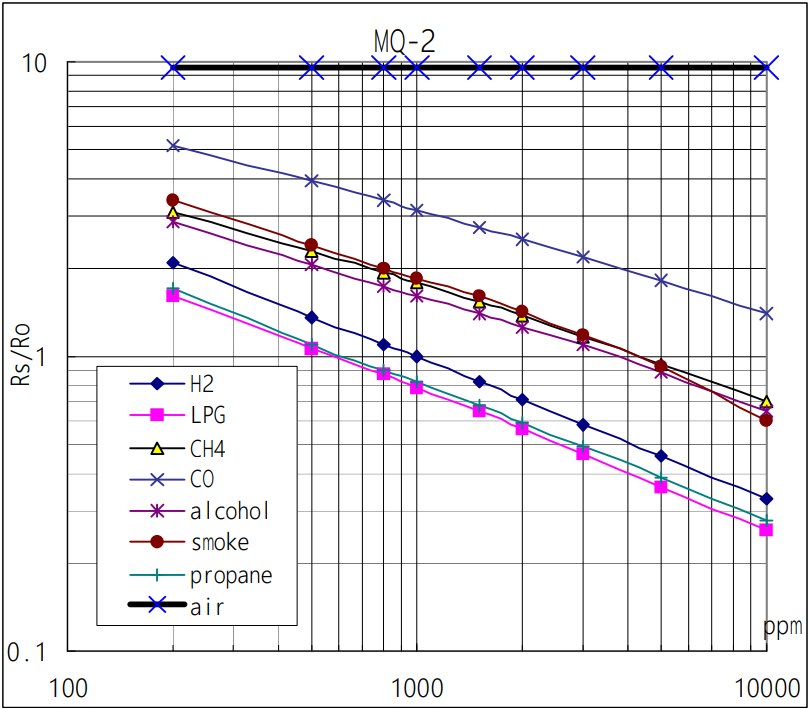
\includegraphics[width=0.8\linewidth]{mq2_sensitivity_characteristics}
    \caption{Typical sensitivity characteristics of the MQ-2 sensor for several gases.}
~\label{fig:mq2_sensitivity_characteristics}
\end{figure}

After calibrating MQ-2 sensor using an Arduino UNO Rev 3 and guide provided by~\cite{grove_2023}, a voltage range value of 0 (for 0ppm) to 1V (10000ppm) is obtained. Load resistor R$_{L}$ was calibrated at 5k$\Omega$. Solving R$_{S}$ from Eq~\ref{eq:voltage_division}:

\begin{equation}
    R_{S} = R_{L} \cdot \frac{V_{out} - V_{S}}{V_{out}}
    \label{eq:r_relationship}
\end{equation}

Substituting V$_{out}$ = 0V and R$_{L}$ = 5k$\Omega$ in Eq~\ref{eq:r_relationship}:

\begin{equation}
    R_{S} ~= \infty \Omega
    \label{eq:rs_at_0v}
\end{equation}

Substituting V$_{out}$ = 1V and R$_{L}$ = 5k$\Omega$ in Eq~\ref{eq:r_relationship}:

\begin{equation}
    R_{S} ~= \infty \Omega
    \label{eq:rs_at_1v}
\end{equation}


\subsubsection{Integration of the System}
~\label{sec:methodology:dev_methodology:iots}
\hspace{8pt}



\begin{figure}[ht]
    \centering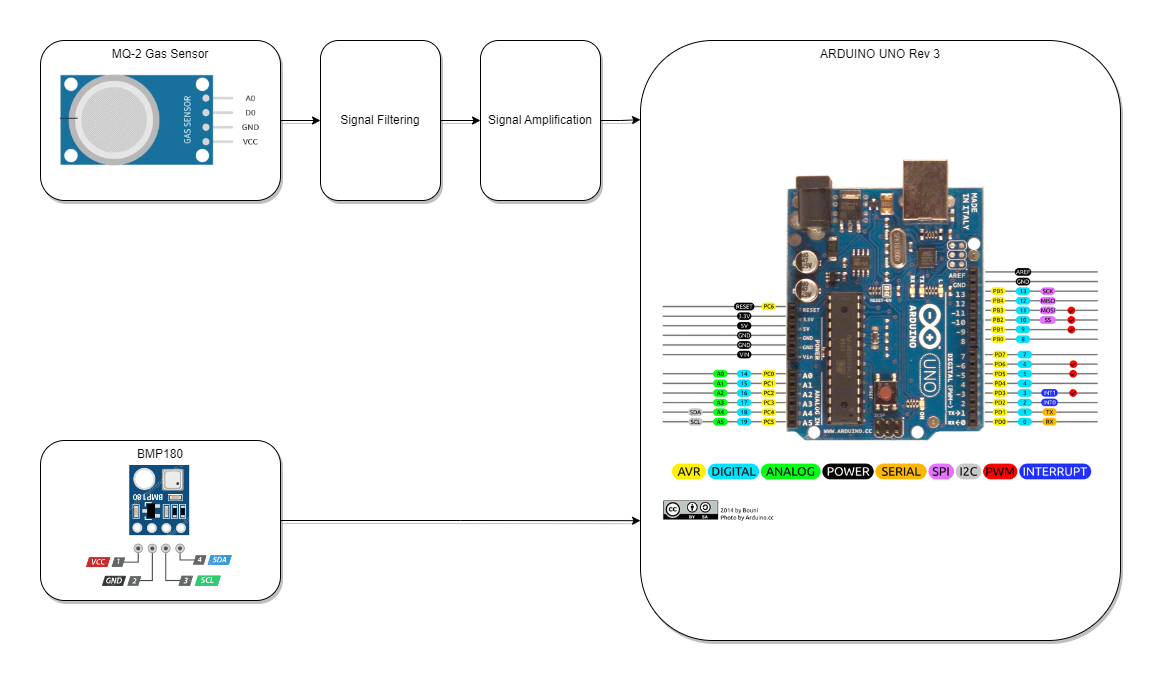
\includegraphics[width=1\linewidth]{integration_of_the_system}
    \caption{Diagram showing the whole system connected.}
~\label{fig:integration_of_the_system}
\end{figure}


\subsubsection{Sampling Algorithm}
~\label{sec:methodology:dev_methodology:sa}
\hspace{8pt}


